One of our central claims is that \pred\ (\gt) internally learns and leverages the shared structure across the training and testing tasks.
% 
To validate this claim, in this section, we consider the introduction of new actions at test time that do \textit{not} follow the structure of training time.
% In this section, we discuss how new actions introduced both during test time and data collection influence the performance of \pred\ (\gt) and other baselines.
%
% These experiments go beyond what is studied in \citet{lee2023supervised, lin2023transformers, ma2023rethinking, liu2023reason} as they only study the performance in setting when $\Dts=\Dpr$. Moreover, 
These experiments are particularly important as they show the extent to which \pred (\gt) is leveraging the latent structure and the shared correlation between the actions and rewards.


\textbf{Invariant actions:} We denote the set of actions fixed across the different tasks in the pretraining in-context dataset as $\Anc$. Therefore these action features $\bx(a)\in\R^d$ for $a\in \Anc$ are fixed across the different tasks $m$. Note that these invariant actions help the transformer $\T_{\bw}$ to learn the latent structure and the reward correlation across the different tasks. Therefore, as the structure breaks down, \pred\ starts performing worse than other baselines.

\textbf{New actions:} We also want to test whether \pred\ (\gt) exploits shared structure when new actions are introduced that are not seen during training time. To this effect, for each task $m\in [\Mpr]$ and $m\in [\Mts]$ we introduce $A - |\Anc|$ new actions. \textit{That is both for train and test tasks, we introduce new actions.}  For each of these new actions $a\in [A - |\Anc|]$ we choose the features $\bx(m,a)$ randomly from $\X\subseteq\R^d$. Note the transformer now trains on a dataset $\H_m \subseteq \Dpr \neq \Dts$.  


% \begin{figure}[!hbt]
% \centering
% \vspace*{-1em}
% \begin{tabular}{cccc}
% \subfigure[Linear $1$ new action]{\hspace*{-1.5em}\includegraphics[scale = 0.1]{img/Neurips/new_arms/linear/lin_1_lr0.00015_do0_embd32_layer4_head4_envs200032_hists1_samples1_var0.3_cov0.0_H51_d12_lind2_seed1_testcov0.0_hor51.pkl.png}\label{fig:new-lin-1}} &
% %%%%%%%%%%
% \subfigure[Non-linear $1$ new action]{\hspace*{-1.5em}\includegraphics[scale = 0.1]{img/Neurips/new_arms/non_linear/nlm_1_shufFalse_lr0.00015_do0_embd32_layer4_head4_envs100001_hists1_samples1_var0.3_cov0.0_H51_d6_lind2_seed1_testcov0.0_hor51.pkl.png} \label{fig:new-nlm-1}} & %\\
% %%%%%%%%%%%%%%%%%%%%%%%
% \subfigure[Linear $5$ new actions]{\hspace*{-1.5em}\includegraphics[scale = 0.1]{img/Neurips/new_arms/linear/lin_5_lr0.00015_do0_embd32_layer4_head4_envs200036_hists1_samples1_var0.3_cov0.0_H51_d12_lind2_seed1_testcov0.0_hor51.pkl.png} \label{fig:new-lin-5}}&
% % %%%%%%%%%%
% \subfigure[Non-linear $5$ new actions]{\hspace*{-1.5em}\includegraphics[scale = 0.1]{img/Neurips/new_arms/non_linear/nlm_5_shufFalse_lr0.00015_do0_embd32_layer4_head4_envs100001_hists1_samples1_var0.3_cov0.0_H51_d6_lind2_seed1_testcov0.0_hor51.pkl.png} \label{fig:new-nlm-5}}
% \end{tabular}
% \vspace*{-1.2em}
% \caption{New action experiments. The horizontal axis is the number of rounds. Confidence bars show one standard error.}
% \label{fig:expt-new-actions}
% \vspace{-0.8em}
% \end{figure}

% \begin{figure}[!hbt]
% \centering
% \vspace*{-1em}
% \begin{tabular}{cccc}
% \subfigure[Linear $0$ new action]{\hspace*{-1.5em}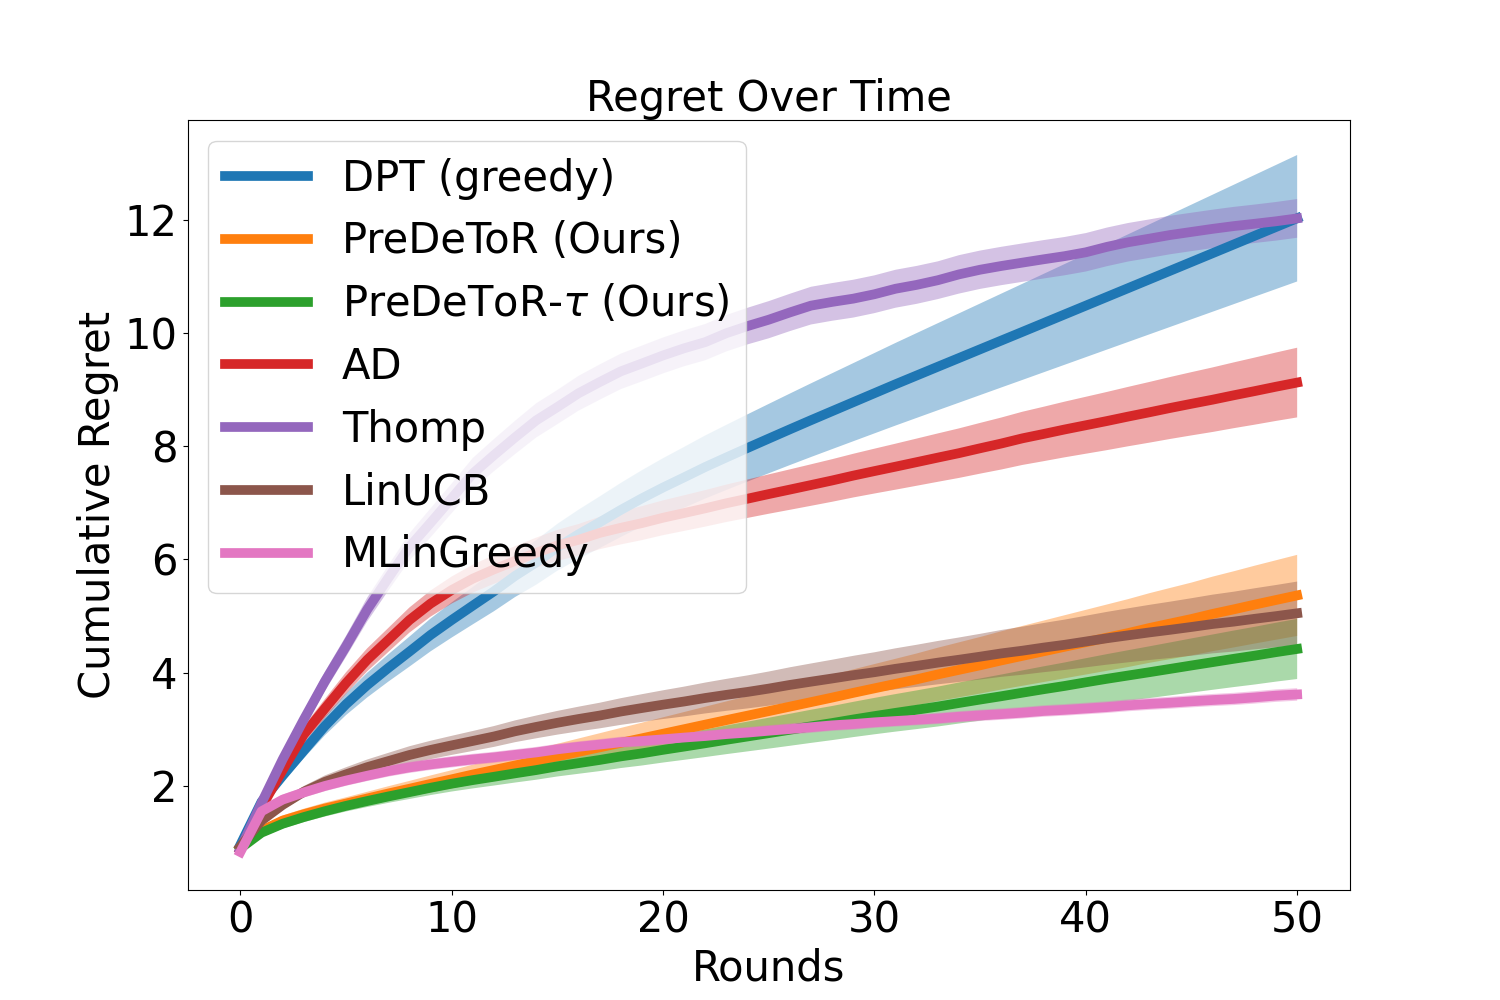
\includegraphics[scale = 0.1]{img/Neurips/new_arms/linear/new/lin1_shufFalse_lr0.00015_do0_embd32_layer4_head4_envs100130_hists1_samples1_var0.3_cov0.0_H51_d10_lind2_seed1_testcov0.0_hor51.pkl.png}\label{fig:new-lin-1}} &
% %%%%%%%%%%
% \subfigure[Linear $1$ new action]{\hspace*{-1.5em}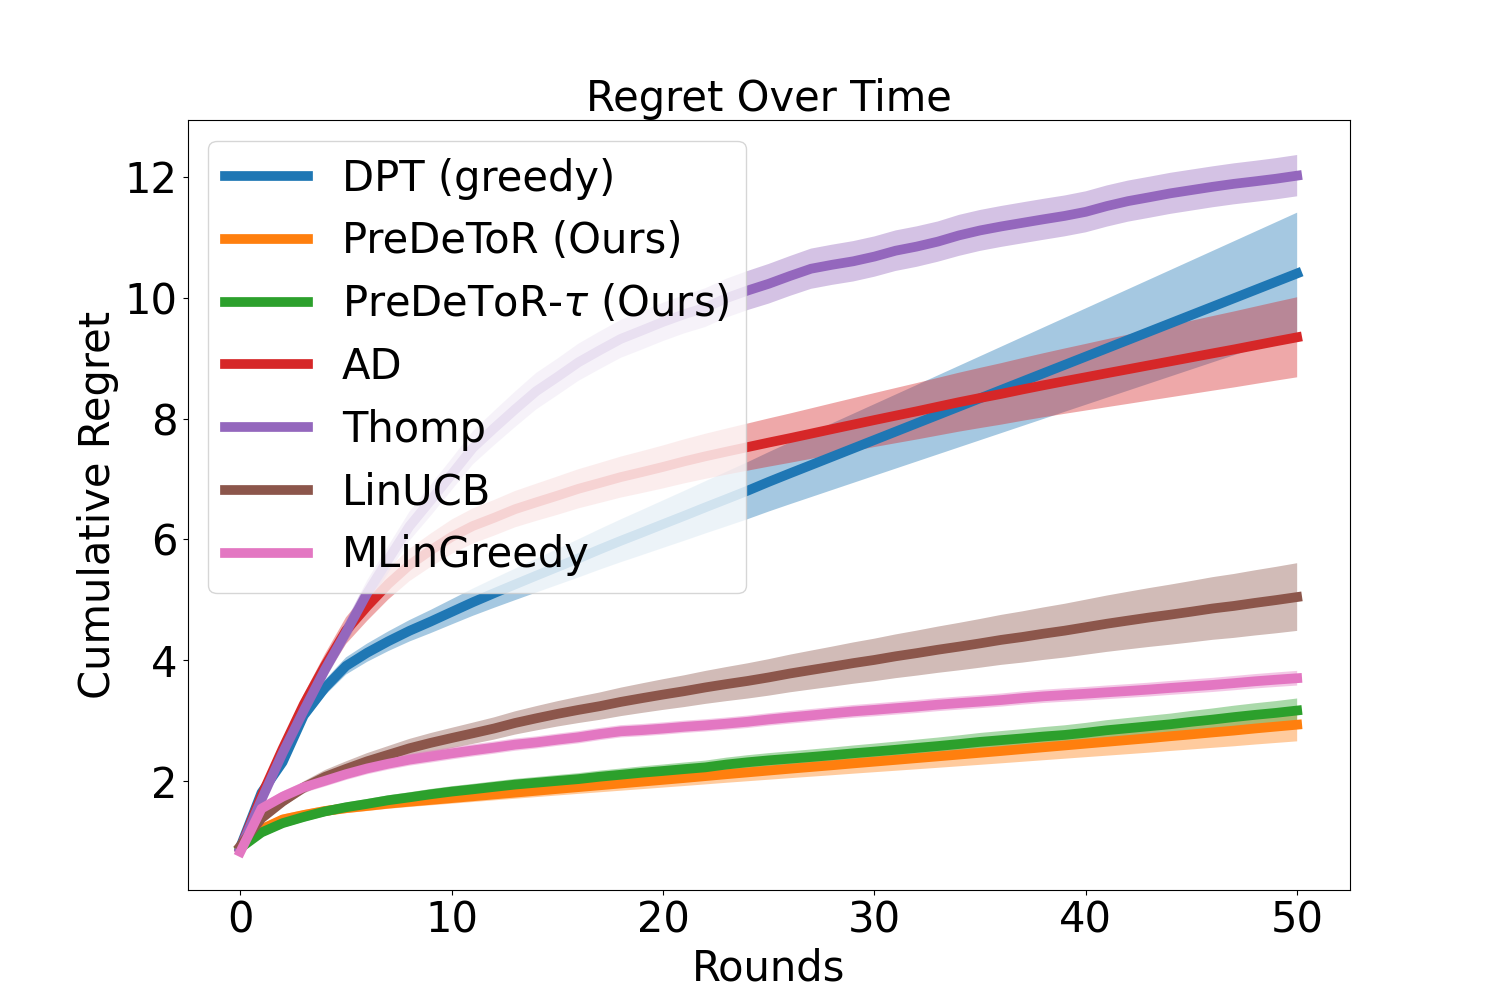
\includegraphics[scale = 0.1]{img/Neurips/new_arms/linear/new/archive/lin2_shufFalse_lr0.00015_do0_embd32_layer4_head4_envs100130_hists1_samples1_var0.3_cov0.0_H51_d10_lind2_seed1_testcov0.0_hor51.pkl.png} \label{fig:new-lin-2}} & %\\
% %%%%%%%%%%%%%%%%%%%%%%%
% \subfigure[Linear $5$ new actions]{\hspace*{-1.5em}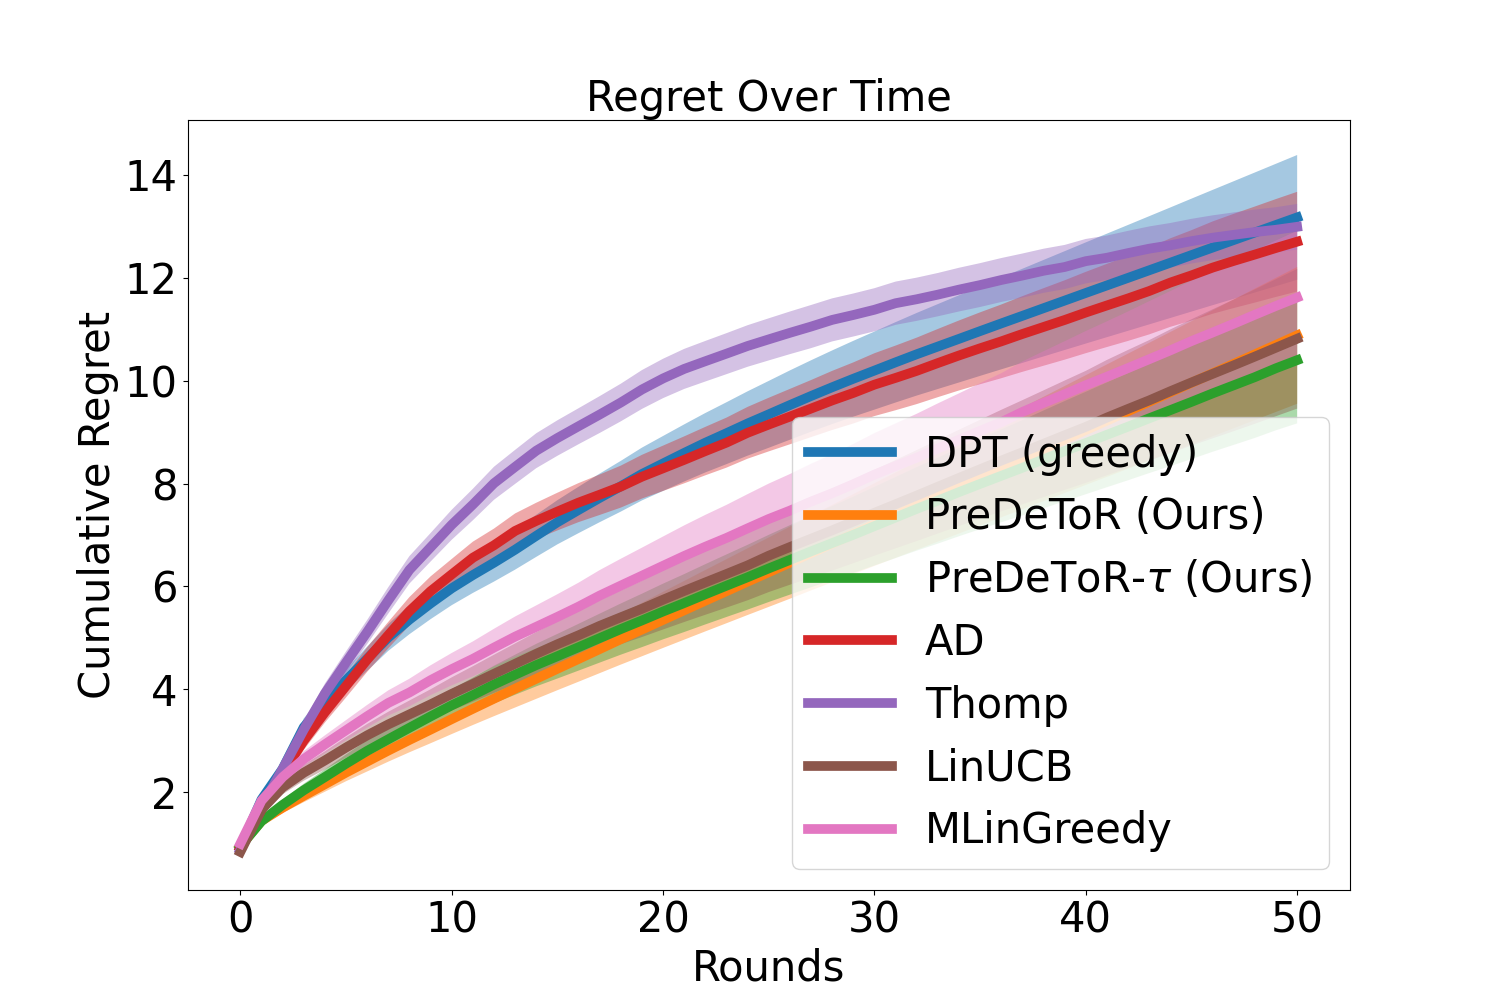
\includegraphics[scale = 0.1]{img/Neurips/new_arms/linear/new/lin3_shufFalse_lr0.00015_do0_embd32_layer4_head4_envs100133_hists1_samples1_var0.3_cov0.0_H51_d10_lind2_seed1_testcov0.0_hor51.pkl.png} \label{fig:new-lin-3}}&
% % %%%%%%%%%%
% \subfigure[Linear $10$ new actions]{\hspace*{-1.5em}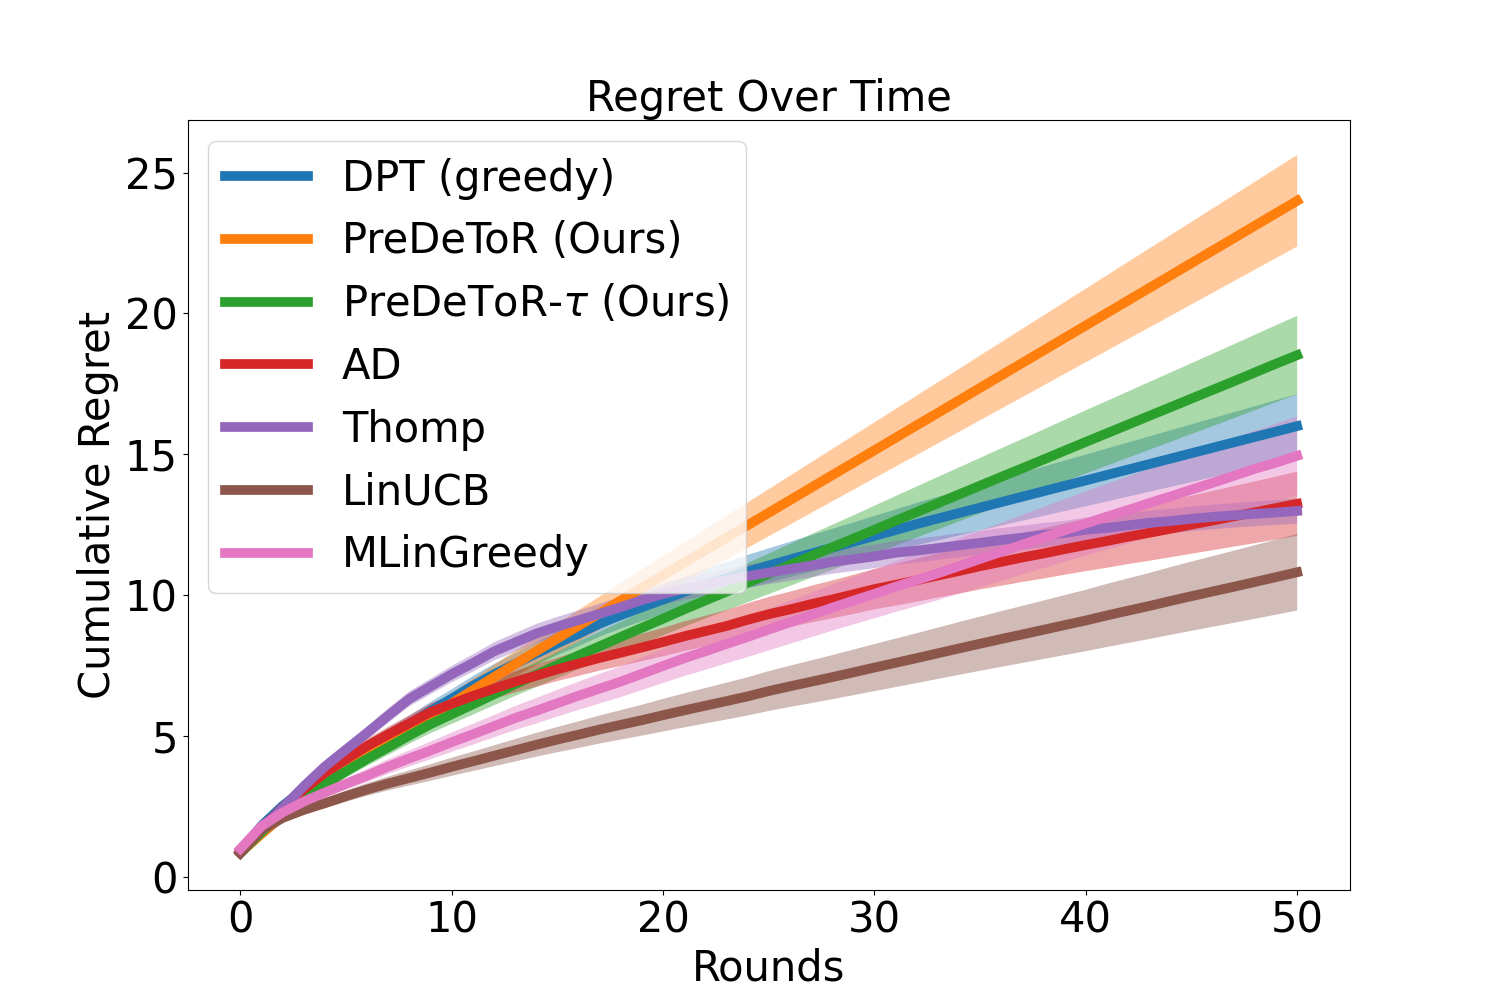
\includegraphics[scale = 0.1]{img/Neurips/new_arms/linear/new/lin4_shufFalse_lr0.00015_do0_embd32_layer4_head4_envs100133_hists1_samples1_var0.3_cov0.0_H51_d10_lind2_seed1_testcov0.0_hor51.pkl.png} \label{fig:new-lin-4}}
% \end{tabular}
% \vspace*{-1.2em}
% \caption{New action experiments. The horizontal axis is the number of rounds. Confidence bars show one standard error.}
% \label{fig:expt-new-actions-lin}
% \vspace{-0.8em}
% \end{figure}


\begin{figure}[!hbt]
\centering
\vspace*{-1em}
\begin{subfigure}[b]{0.24\textwidth}
    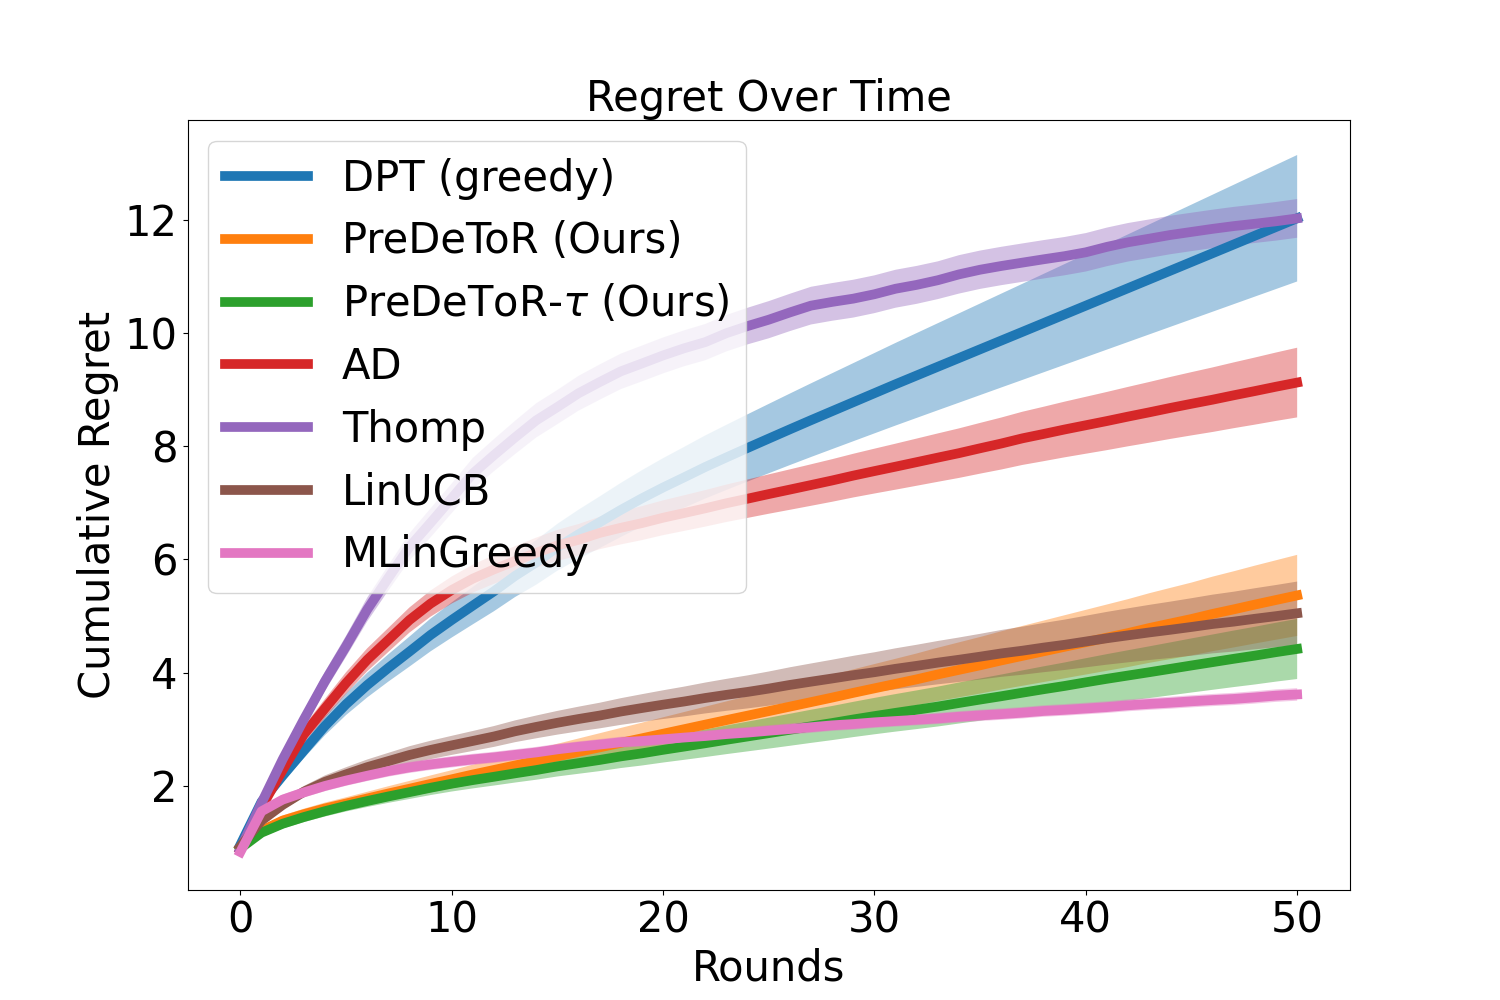
\includegraphics[scale=0.1]{img/Neurips/new_arms/linear/new/lin1_shufFalse_lr0.00015_do0_embd32_layer4_head4_envs100130_hists1_samples1_var0.3_cov0.0_H51_d10_lind2_seed1_testcov0.0_hor51.pkl.png}
    \caption{$0$ new action}
    \label{fig:new-lin-1}
\end{subfigure}%
\begin{subfigure}[b]{0.24\textwidth}
    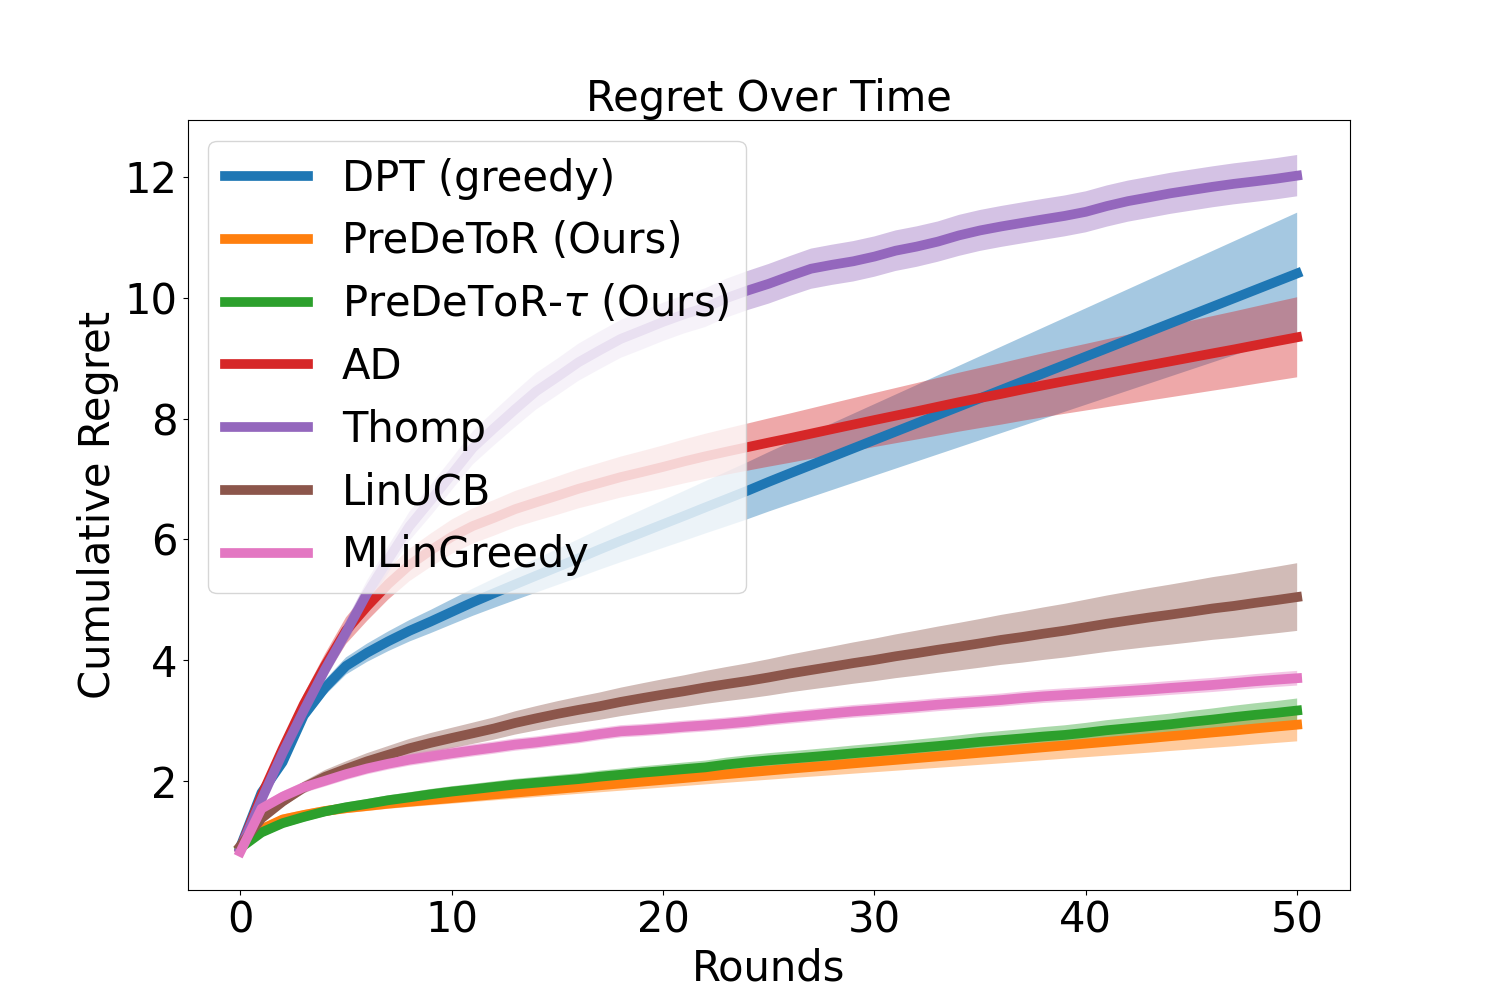
\includegraphics[scale=0.1]{img/Neurips/new_arms/linear/new/archive/lin2_shufFalse_lr0.00015_do0_embd32_layer4_head4_envs100130_hists1_samples1_var0.3_cov0.0_H51_d10_lind2_seed1_testcov0.0_hor51.pkl.png}
    \caption{$1$ new action}
    \label{fig:new-lin-2}
\end{subfigure}%
\begin{subfigure}[b]{0.24\textwidth}
    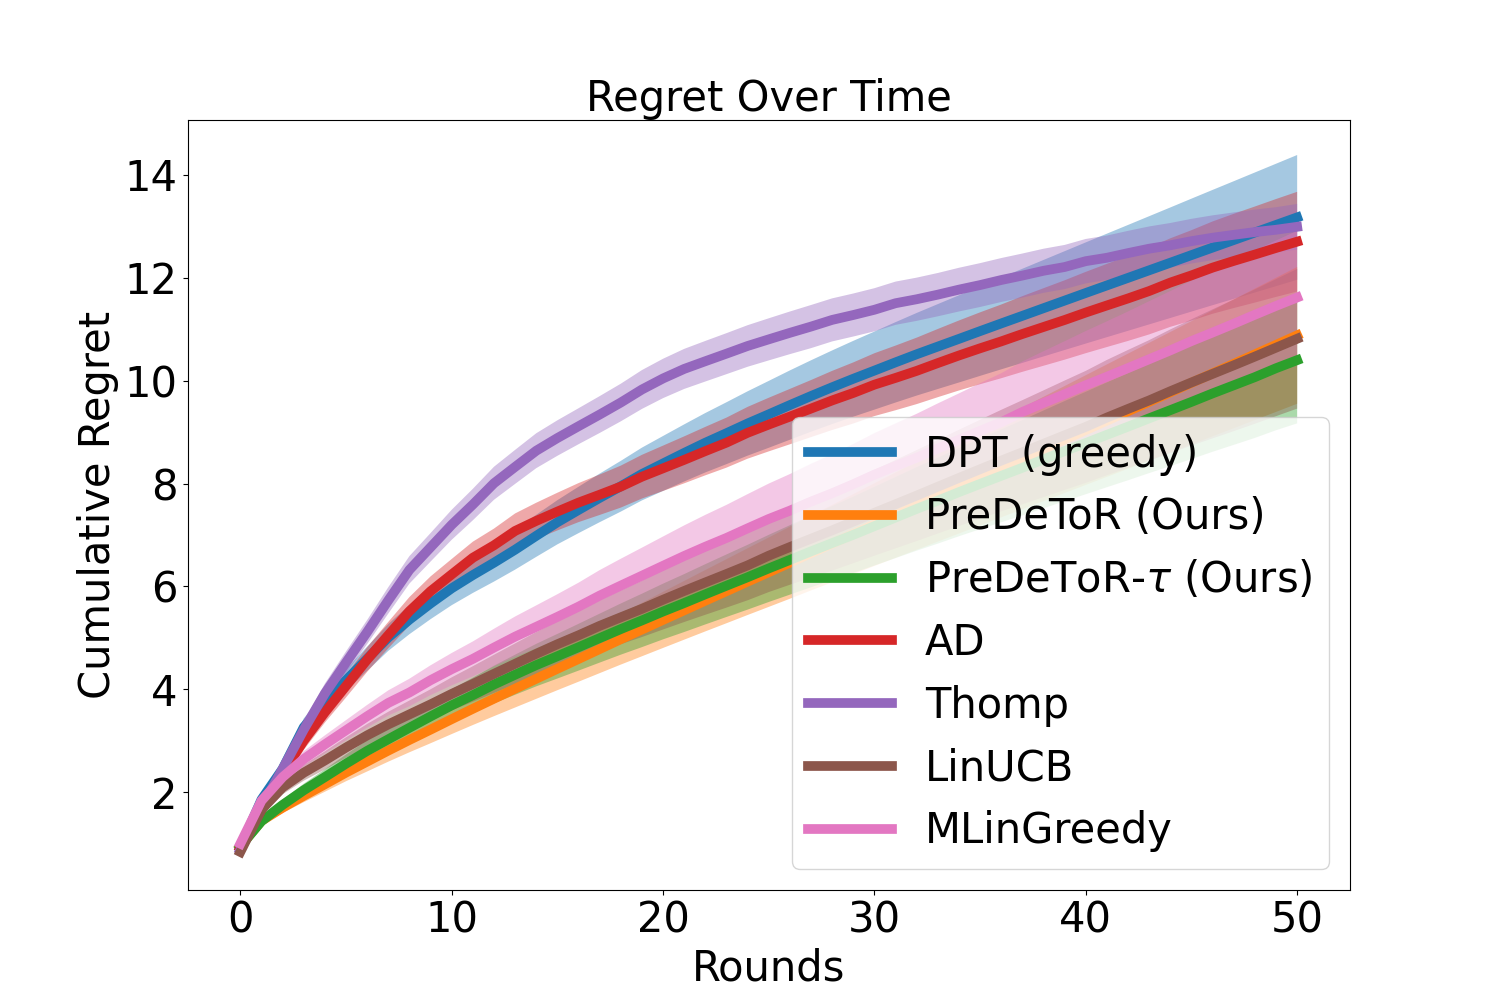
\includegraphics[scale=0.1]{img/Neurips/new_arms/linear/new/lin3_shufFalse_lr0.00015_do0_embd32_layer4_head4_envs100133_hists1_samples1_var0.3_cov0.0_H51_d10_lind2_seed1_testcov0.0_hor51.pkl.png}
    \caption{$5$ new actions}
    \label{fig:new-lin-3}
\end{subfigure}%
\begin{subfigure}[b]{0.24\textwidth}
    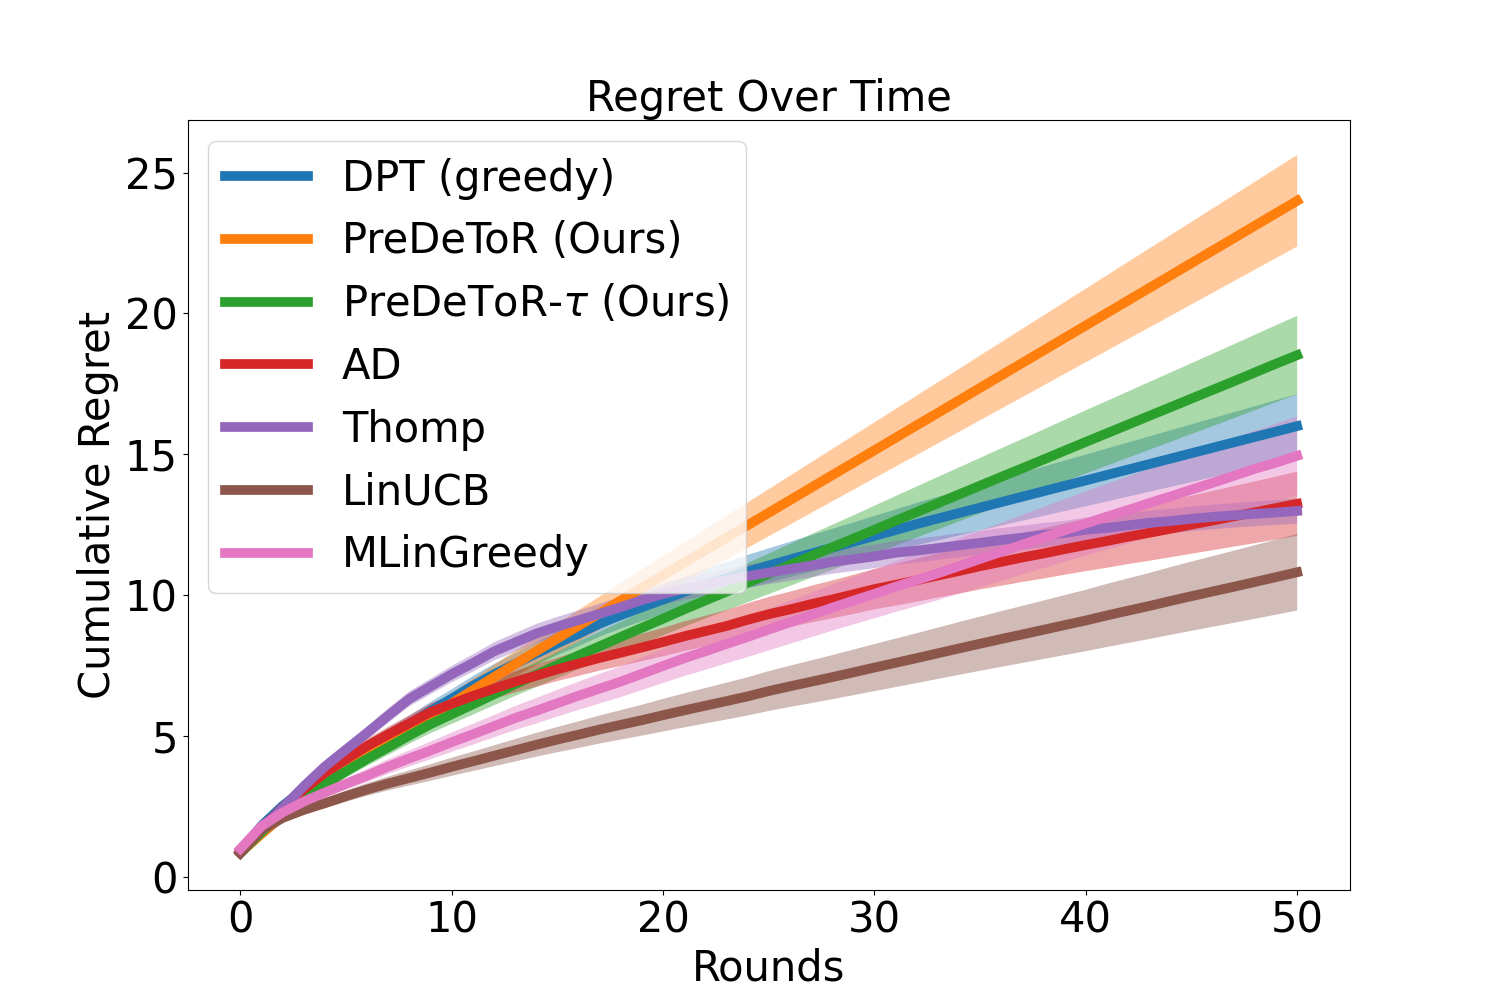
\includegraphics[scale=0.1]{img/Neurips/new_arms/linear/new/lin4_shufFalse_lr0.00015_do0_embd32_layer4_head4_envs100133_hists1_samples1_var0.3_cov0.0_H51_d10_lind2_seed1_testcov0.0_hor51.pkl.png}
    \caption{$10$ new actions}
    \label{fig:new-lin-4}
\end{subfigure}
\vspace*{-1.2em}
\caption{Linear new action experiments. The horizontal axis is the number of rounds. Confidence bars show one standard error.}
\label{fig:expt-new-actions-lin}
\vspace{-0.8em}
\end{figure}

% \begin{figure}[!hbt]
% \centering
% \vspace*{-1em}
% \begin{tabular}{cccc}
% \subfigure[Non-linear $0$ new action]{\hspace*{-1.5em}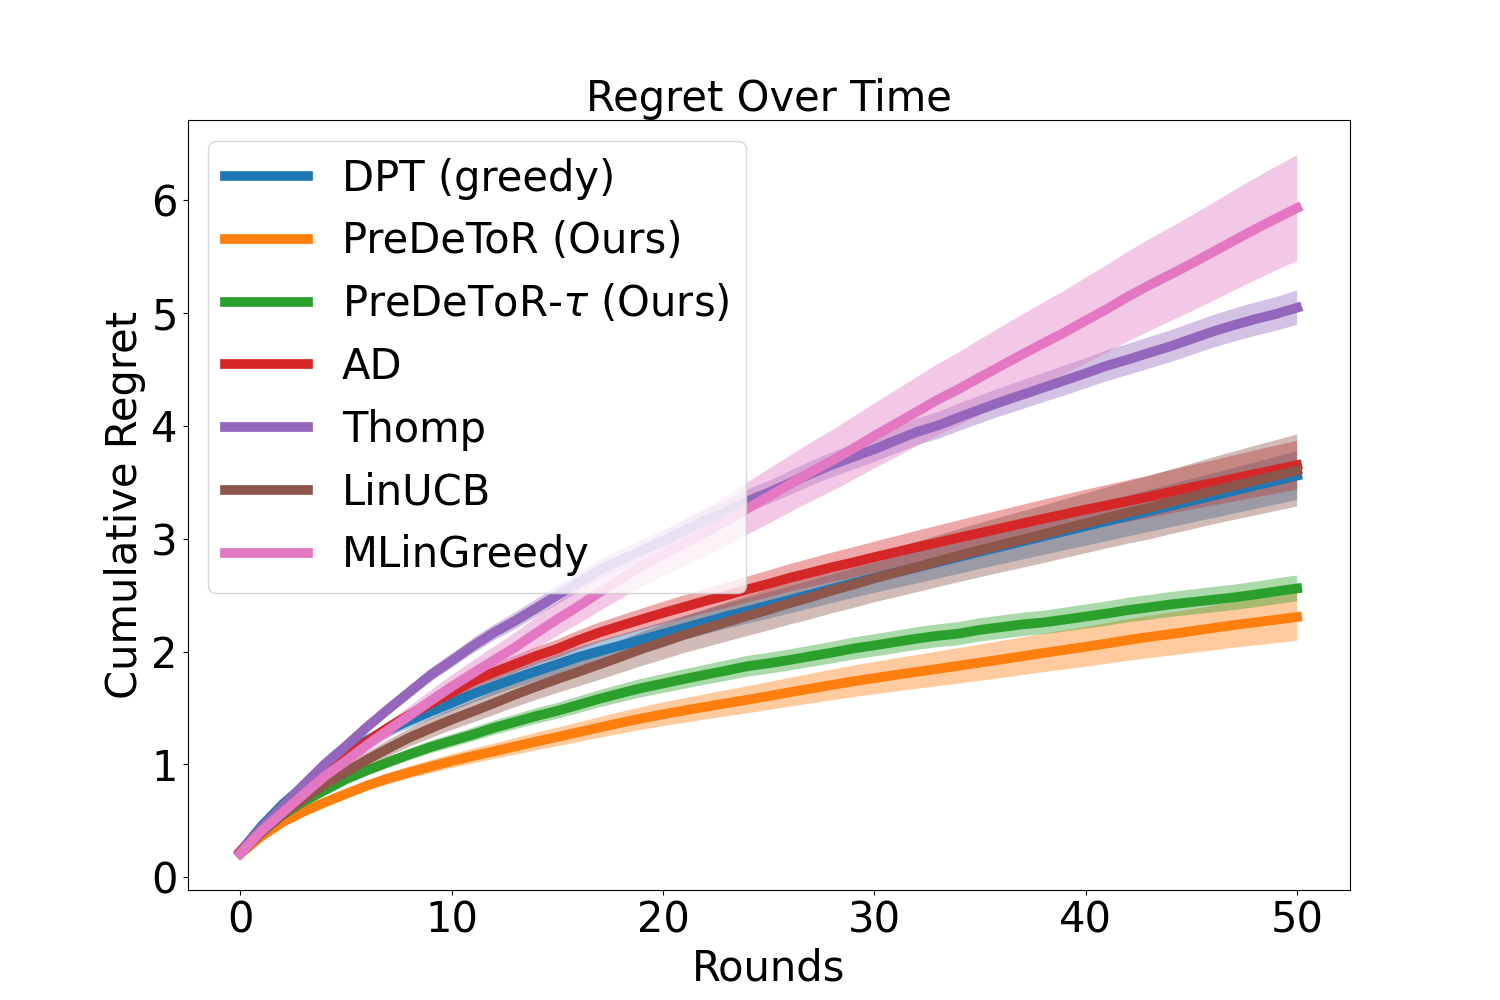
\includegraphics[scale = 0.1]{img/Neurips/new_arms/linear/new/nlm1_shufFalse_lr0.00015_do0_embd32_layer4_head4_envs100130_hists1_samples1_var0.3_cov0.0_H51_d10_lind2_seed1_testcov0.0_hor51.pkl.png}\label{fig:new-nlm-1}} &
% %%%%%%%%%%
% \subfigure[Non-linear $1$ new action]{\hspace*{-1.5em}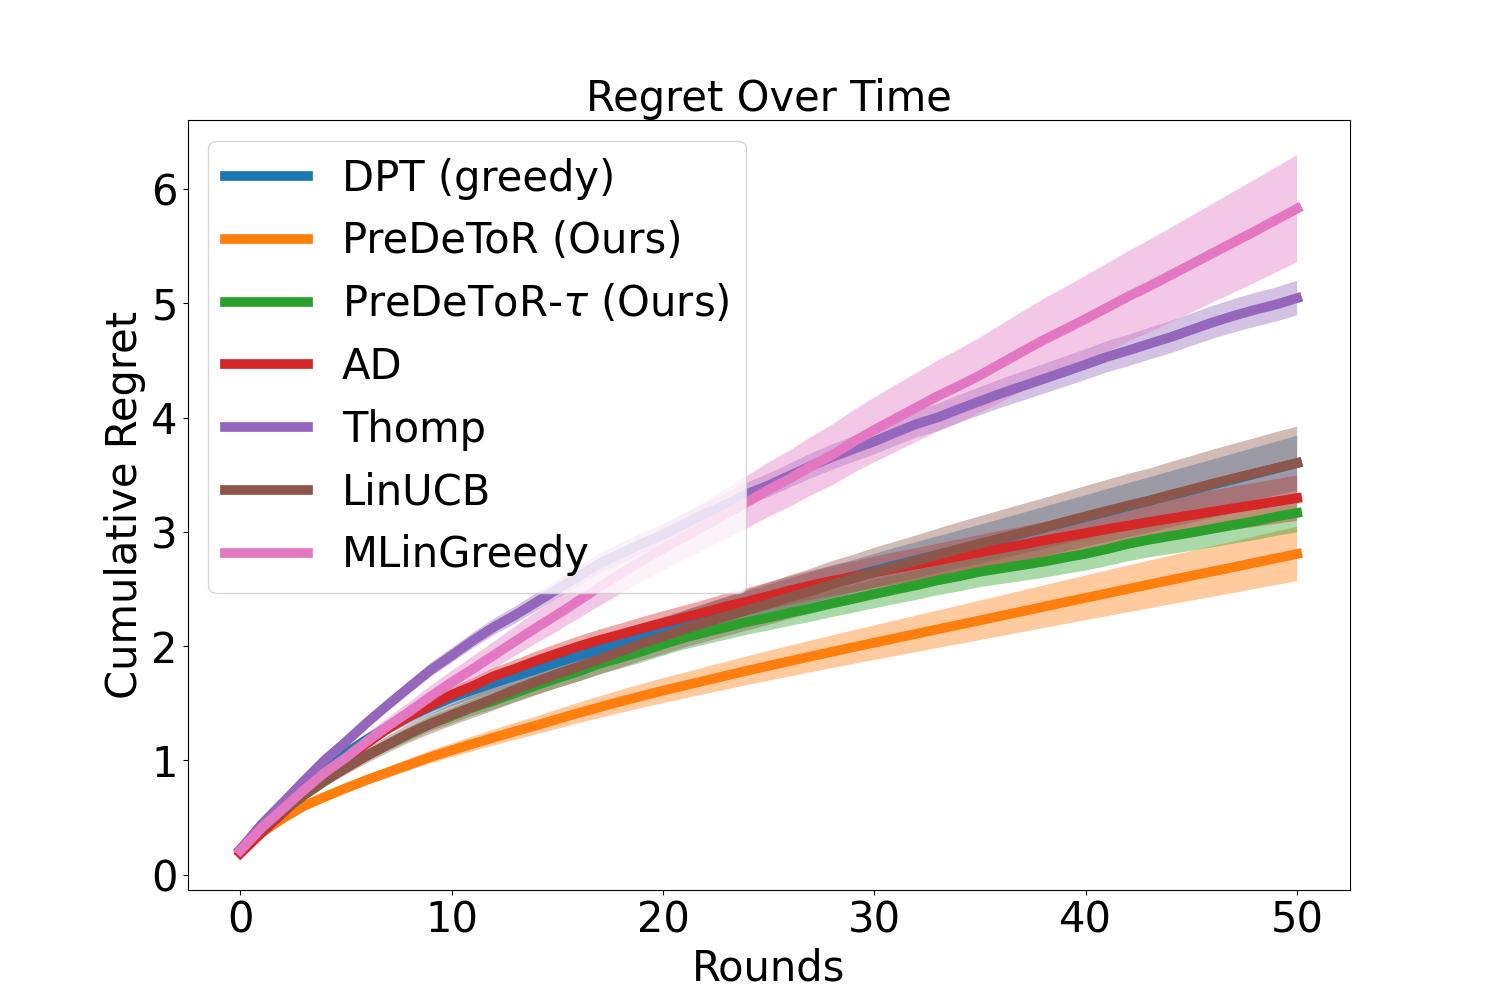
\includegraphics[scale = 0.1]{img/Neurips/new_arms/linear/new/nlm2_shufFalse_lr0.00015_do0_embd32_layer4_head4_envs100130_hists1_samples1_var0.3_cov0.0_H51_d10_lind2_seed1_testcov0.0_hor51.pkl.png} \label{fig:new-nlm-2}} & %\\
% %%%%%%%%%%%%%%%%%%%%%%%
% \subfigure[Non-linear $5$ new actions]{\hspace*{-1.5em}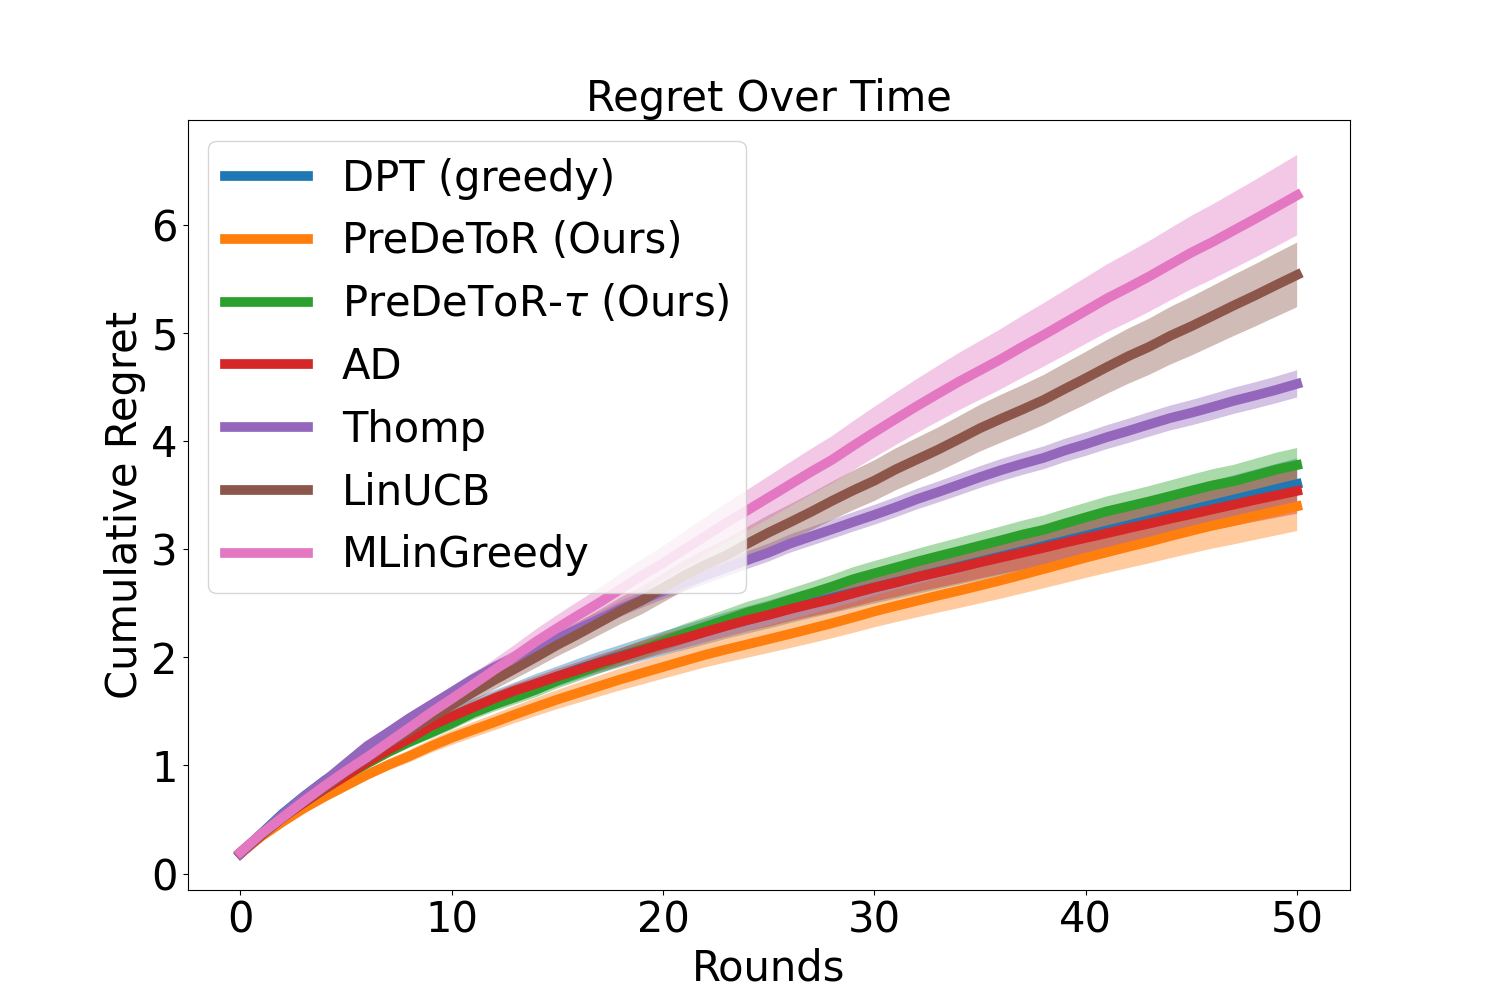
\includegraphics[scale = 0.1]{img/Neurips/new_arms/linear/new/nlm3_shufFalse_lr0.00015_do0_embd32_layer4_head4_envs100130_hists1_samples1_var0.3_cov0.0_H51_d10_lind2_seed1_testcov0.0_hor51.pkl.png} \label{fig:new-nlm-3}}&
% % %%%%%%%%%%
% \subfigure[Non-linear $10$ new actions]{\hspace*{-1.5em}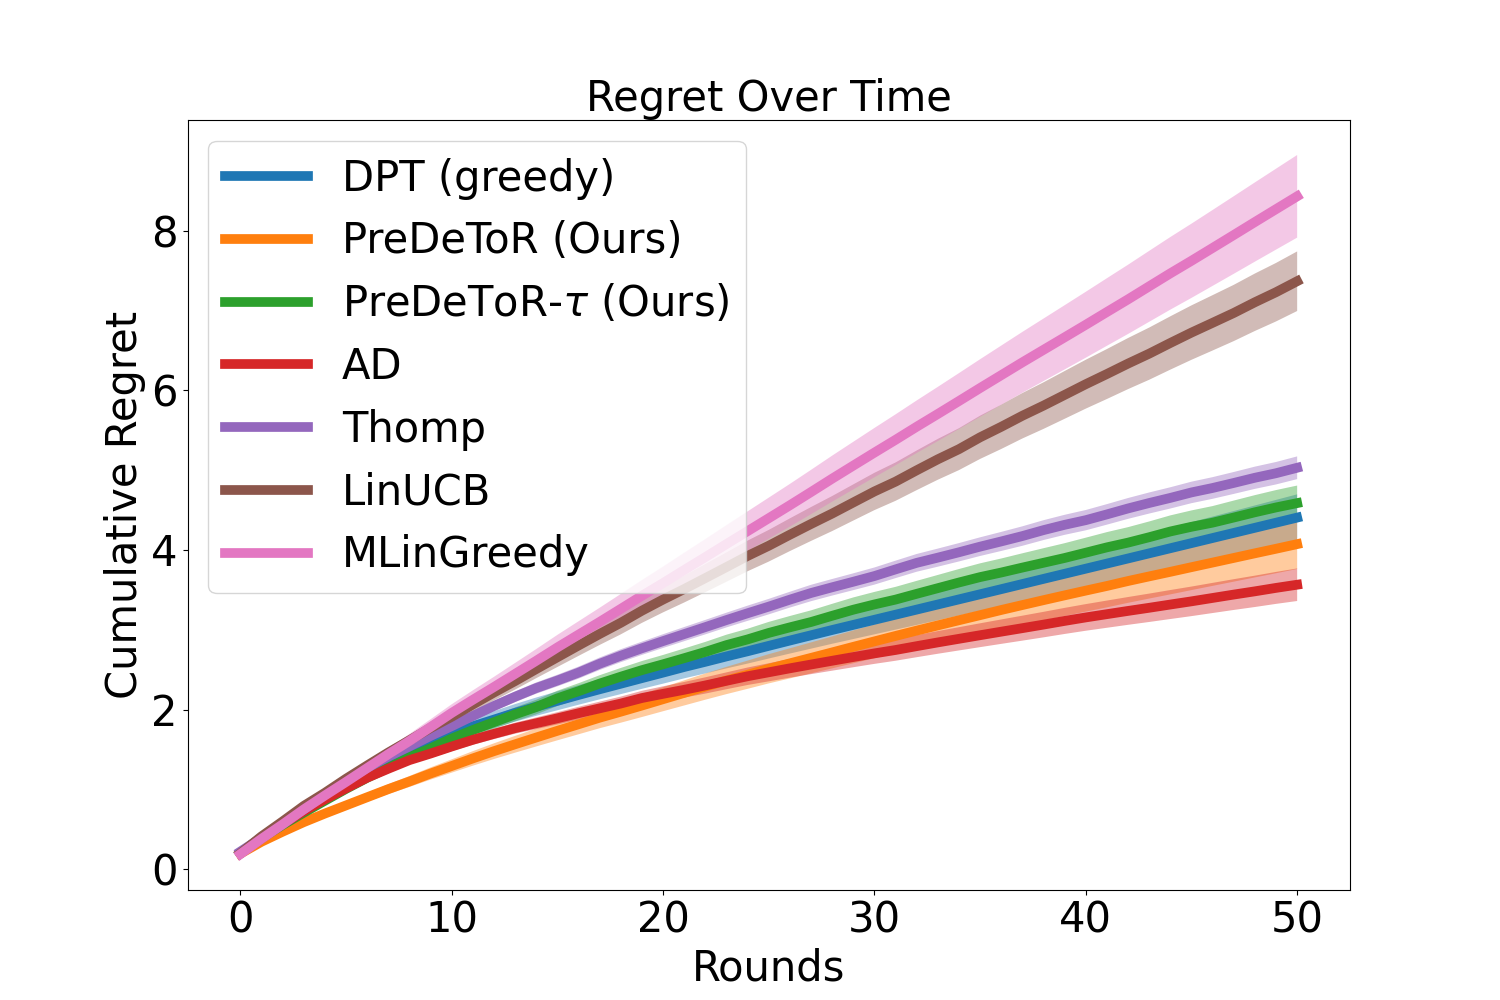
\includegraphics[scale = 0.1]{img/Neurips/new_arms/linear/new/nlm4_shufFalse_lr0.00015_do0_embd32_layer4_head4_envs100130_hists1_samples1_var0.3_cov0.0_H51_d10_lind2_seed1_testcov0.0_hor51.pkl.png} \label{fig:new-nlm-4}}
% \end{tabular}
% \vspace*{-1.2em}
% \caption{New action experiments with non-linear setting. 
% % The horizontal axis is the number of rounds. Confidence bars show one standard error.
% }
% \label{fig:expt-new-actions-nlm}
% \vspace{-0.8em}
% \end{figure}


\begin{figure}[!hbt]
\centering
\vspace*{-1em}
\begin{subfigure}[b]{0.24\textwidth}
    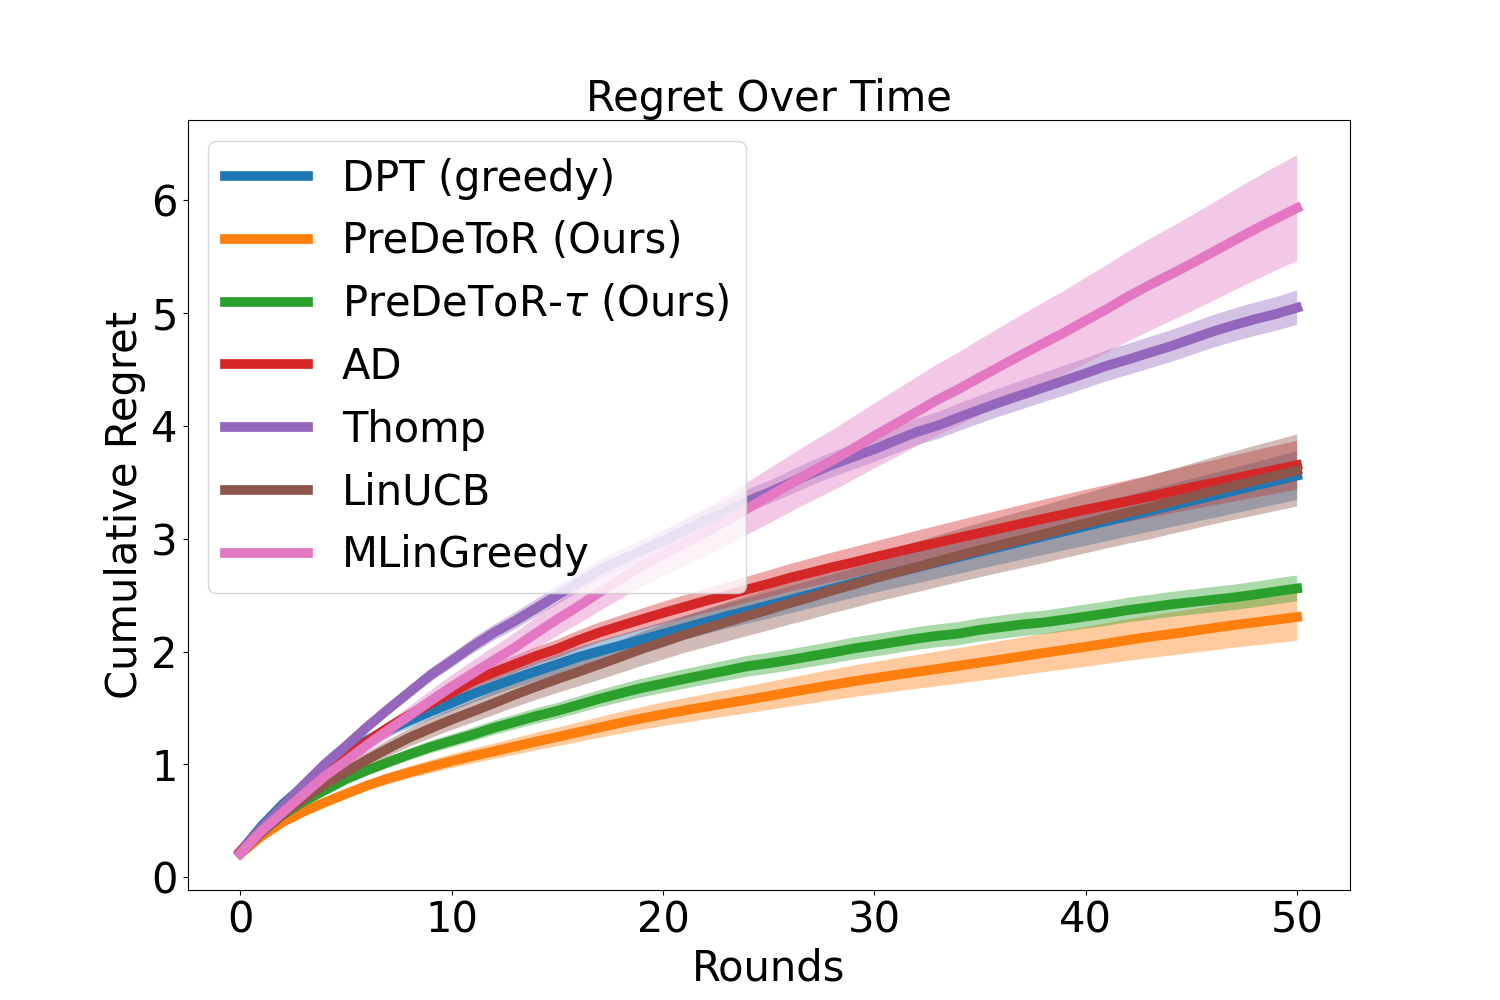
\includegraphics[scale=0.1]{img/Neurips/new_arms/linear/new/nlm1_shufFalse_lr0.00015_do0_embd32_layer4_head4_envs100130_hists1_samples1_var0.3_cov0.0_H51_d10_lind2_seed1_testcov0.0_hor51.pkl.png}
    \caption{$0$ new action}
    \label{fig:new-nlm-1}
\end{subfigure}%
\begin{subfigure}[b]{0.24\textwidth}
    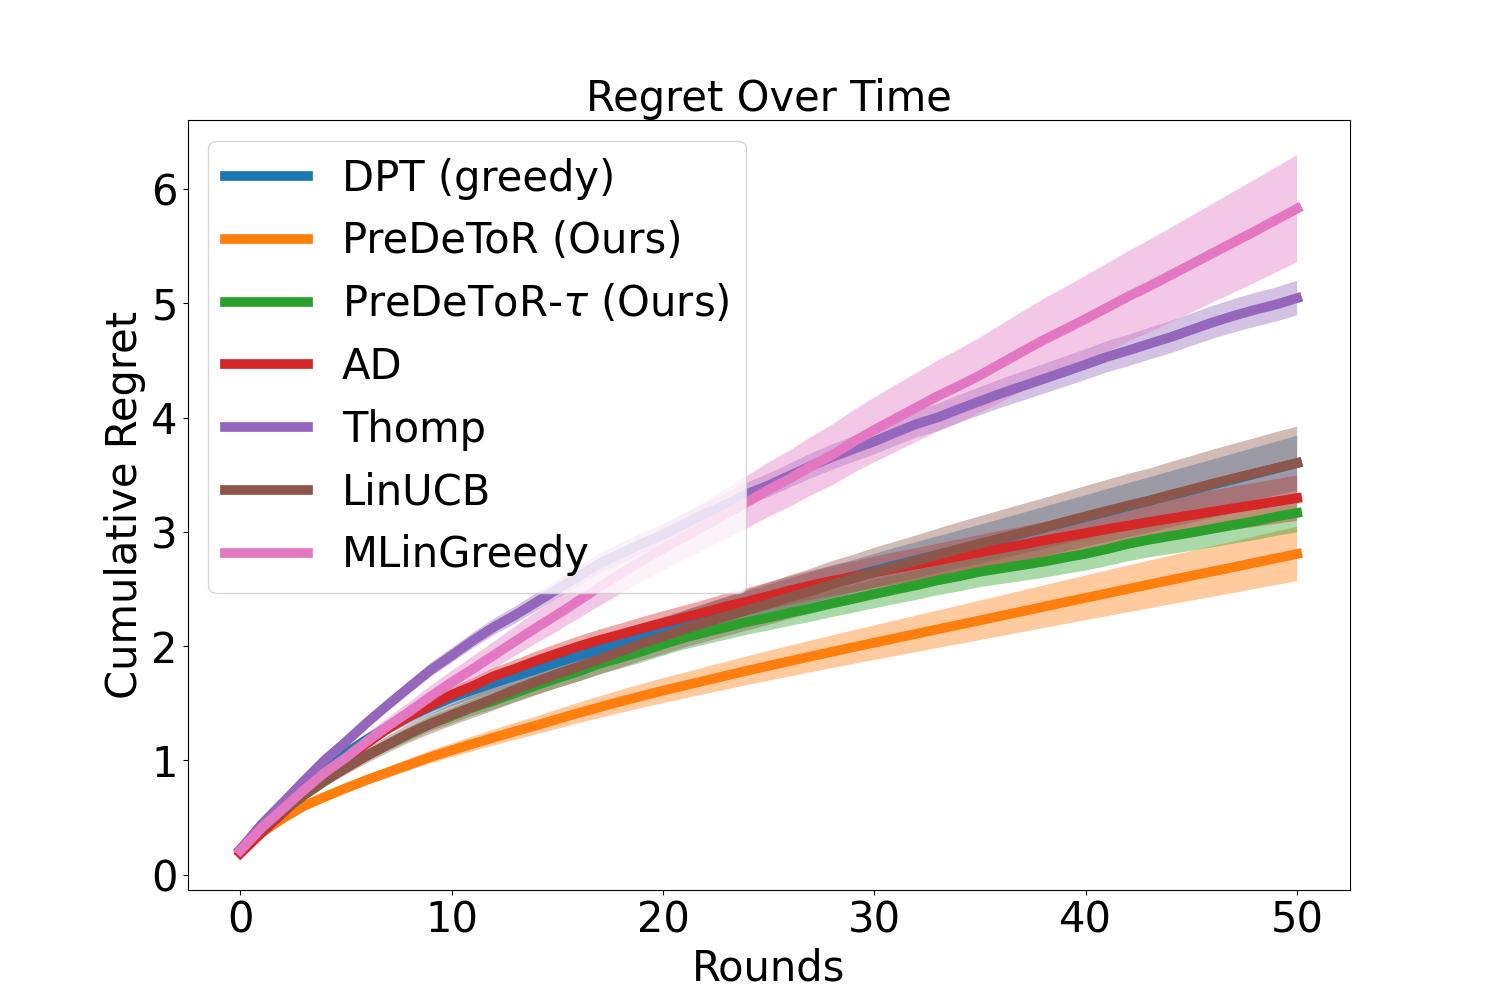
\includegraphics[scale=0.1]{img/Neurips/new_arms/linear/new/nlm2_shufFalse_lr0.00015_do0_embd32_layer4_head4_envs100130_hists1_samples1_var0.3_cov0.0_H51_d10_lind2_seed1_testcov0.0_hor51.pkl.png}
    \caption{$1$ new action}
    \label{fig:new-nlm-2}
\end{subfigure}%
\begin{subfigure}[b]{0.24\textwidth}
    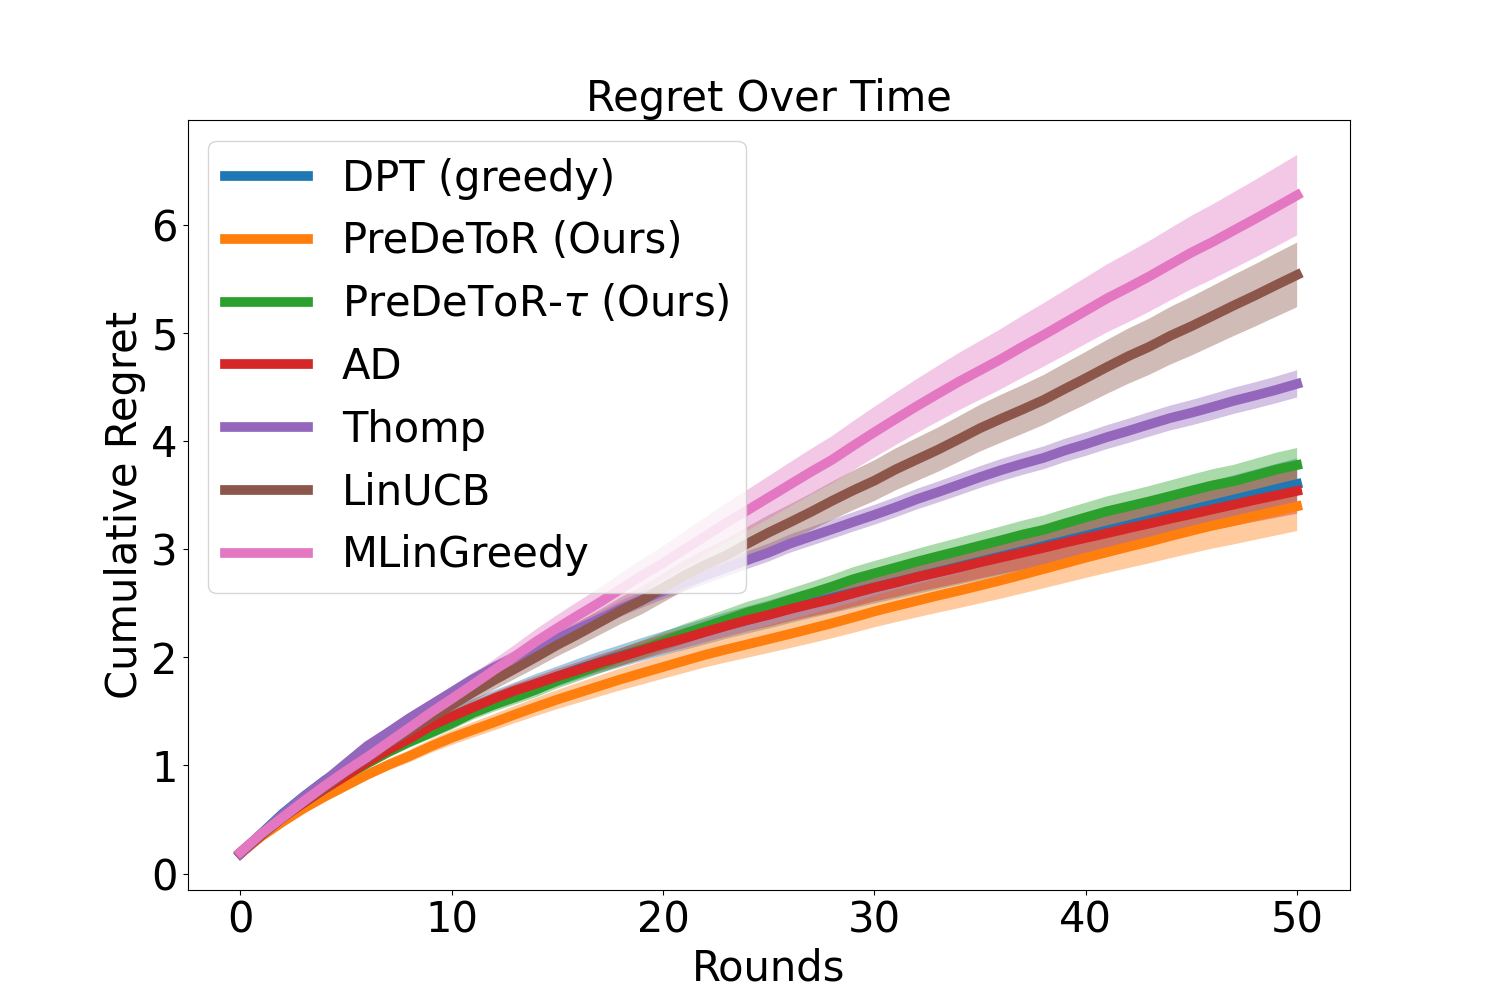
\includegraphics[scale=0.1]{img/Neurips/new_arms/linear/new/nlm3_shufFalse_lr0.00015_do0_embd32_layer4_head4_envs100130_hists1_samples1_var0.3_cov0.0_H51_d10_lind2_seed1_testcov0.0_hor51.pkl.png}
    \caption{$5$ new actions}
    \label{fig:new-nlm-3}
\end{subfigure}%
\begin{subfigure}[b]{0.24\textwidth}
    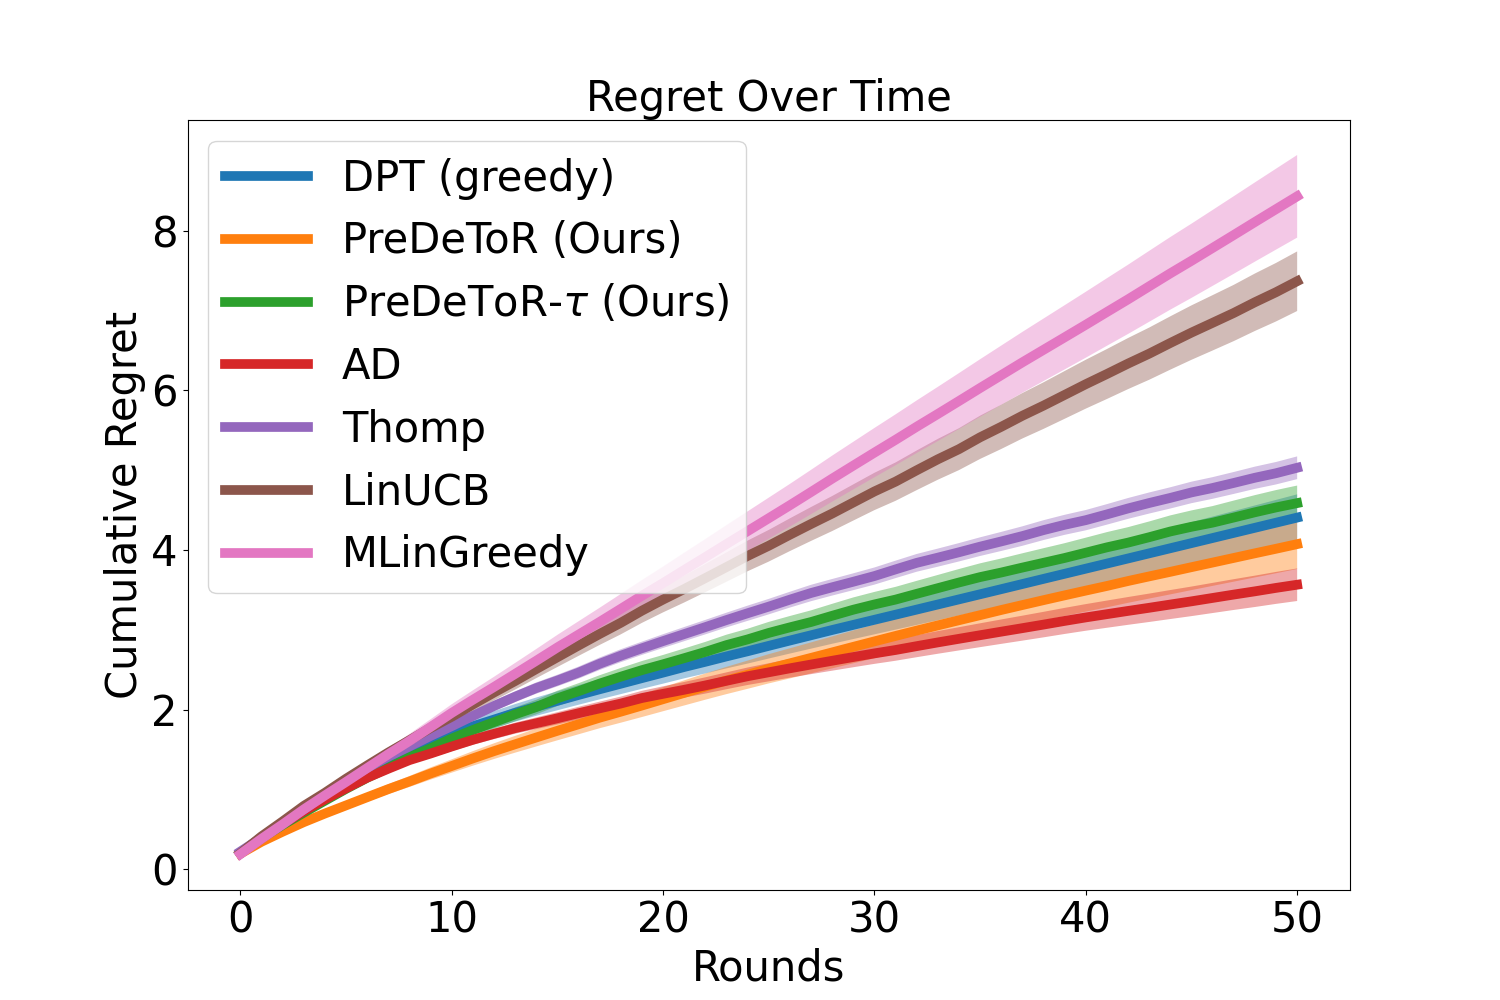
\includegraphics[scale=0.1]{img/Neurips/new_arms/linear/new/nlm4_shufFalse_lr0.00015_do0_embd32_layer4_head4_envs100130_hists1_samples1_var0.3_cov0.0_H51_d10_lind2_seed1_testcov0.0_hor51.pkl.png}
    \caption{$10$ new actions}
    \label{fig:new-nlm-4}
\end{subfigure}
\vspace*{-1.2em}
\caption{Non-linear new action experiments with non-linear setting.}
\label{fig:expt-new-actions-nlm}
\vspace{-0.8em}
\end{figure}

\textbf{Baselines:} We implement the same baselines discussed in \Cref{sec:short-horizon}. 
% The baselines are \pred, \predt, \dptg, \ad, \ts, and \linucb. 


\textbf{Outcomes:} Again before presenting the result we discuss the main outcomes from our experimental results of introducing new actions during data collection and evaluation:

\begin{tcolorbox}
\customfinding Shared structure across the tasks is important to learn the reward structure. 
\end{tcolorbox}


% \noindent
% \textbf{(1)} The \pred\ (\gt) learns to exploit the underlying latent structure and reward correlation between the different tasks even when $\Dts\neq\Dpr$ and the number of changing actions per task is small. 
% % So \pred\ (\gt) is more robust to changing actions compared to \ad\ and \dptg.   

% \textbf{(2)} \pred\ (\gt) has lower regret than weak demonstrator even when it is trained on $\Dpr\neq \Dts$.

%  \textbf{(3)} The \pred\ (\gt) cumulative regret increases as the number of invariant actions decreases. This shows that invariant actions are important for learning the underlying latent structure and reward correlation across tasks.


\textbf{Experimental Result:} We observe these outcomes in \Cref{fig:expt-new-actions-lin} and \Cref{fig:expt-new-actions-nlm}. We consider the linear and non-linear bandit setting of horizon $n=50$, $\Mpr = 100000$, $\Mts = 200$, $A=10$, and $d=2$. 
%
Here during data collection and during collecting the test data, we randomly select between $0, 1, 5$, and $10$ new actions from $\R^d$ for each task $m$. 
%
So the number of invariant actions is $|\Anc| \in \{10, 5, 1, 0\}$. 
%
Again, the demonstrator $\pi^w$ is the \ts\ algorithm. From \Cref{fig:new-lin-1}, \ref{fig:new-lin-2}, \ref{fig:new-lin-3}, and \ref{fig:new-lin-4}, we observe that when the number of invariant actions is less than \pred\ (\gt) has lower cumulative regret than \dptg, and \ad. 
% Moreover \pred\ matches the performance of \linucb. 
%
% The weak performance of \dptg\ can be attributed to low data per task and inability to adapt when $\Dpr\neq\Dts$. 
%
%Note that for this small horizon setting the \dptg\ does not have a good estimation of $\widehat{a}_{m,*}$ which results in a poor prediction of optimal action $\widehat{a}_{m,t,*}$. 
% This results in higher regret. 
Observe that \pred\ (\gt) matches \linucb\ and has lower regret than \dptg, and \ad\ when $\Anc| \in \{10, 5, 1\}$. This shows that \pred\ (\gt) is able to exploit the latent linear structure of the underlying tasks. However, as the number of invariant actions decreases we see that \pred (\gt) performance drops and becomes similar to the unstructured bandits \ts. We also show in \Cref{sec:k_arms_dpt} that in $K$-armed bandit setting when there is no structure across arms \pred\ (\gt) matches the performance of the demonstrator. 
%

Similarly in \Cref{fig:new-nlm-1}, \ref{fig:new-nlm-2}, \ref{fig:new-nlm-3}, and \ref{fig:new-nlm-4} we show the performance of \pred\ in the non-linear bandit setting. Observe that \linucb, \mlin\ fails to perform well in this non-linear setting due to their assumption of linear rewards. Again note that \pred\ (\gt) has lower regret than \dptg, and \ad\ when $\Anc| \in \{10, 1\}$. This shows that \pred\ (\gt) is able to exploit the latent linear structure of the underlying tasks. However, as the number of invariant actions decreases we see that \pred (\gt) performance drops and becomes similar to \ad.


% In \Cref{fig:new-nlm-1} we show the non-linear bandit setting for horizon $n=50$, $\Mpr = 100000$, $\Mts = 200$, $A=6$, $d=2$, and $|\Anc|=5$. The demonstrator $\pi^w$ is the \ts\ algorithm. 
% We observe that \ad\ is not able to outperform its demonstrator \ts\ as it is trained to predict the next action of the demonstrator. 
% Again, we observe that \pred\ has lower cumulative regret than \dptg\ and \ad\ and furthermore improves upon \linucb\ which fails to perform well in this non-linear setting due to its assumption of linear rewards. \predt\ performs slightly better than \pred\ in $1$ new arm setting as it conducts more exploration.

% In the following two experiments, we test the robustness of \pred\ (\gt) by decreasing the number of invariant actions. We use $|\Anc| = 15$ for linear, and $|\Anc| = 2$ for the non-linear setting. All the other task parameters are the same as in the previous two experiments. The corresponding results are shown in \Cref{fig:new-lin-5} and \Cref{fig:new-nlm-5}. Observe that in the linear setting (where \linucb\ is effective), the performance of \pred\ degrades compared to the case when $|\Anc| = 15$. This shows that as the number of invariant actions decreases, the ability of \pred\ (\gt) to estimate the underlying latent structure and reward correlation also decreases. In \Cref{sec:new-arms-app}, we analyze the exploration of \pred\ (\gt) in this setting, which shows that the shared latent structure is essential for minimizing cumulative regret.

% We also empirically study the test performance of \pred\ (\gt) in other \textit{non-linear} bandit settings such as bilinear bandits (\Cref{sec:bilinear}), latent bandits (\Cref{sec:latent}), draw a connection between \pred\ and Bayesian estimators (\Cref{sec:und}), and perform sensitivity and ablation studies in \Cref{sec:lim}, \ref{sec:dimension}, \ref{sec:heads}, \ref{sec:envs}. We discuss data collection algorithms in \Cref{sec:data-collection} and the offline setting in \Cref{sec:offline}. Due to space constraints, we refer the interested reader to the relevant section in the appendices.
%





% Due to space constraints, we refer the interested reader to the Appendix.
% We also study the bilinear bandit setting in \Cref{sec:bilinear}, latent bandit setting in \Cref{sec:latent}. 
% %
% We draw connection between \pred\ and Bayesian estimators in \Cref{sec:und}.
% %
% We study the increasing action setting in \Cref{sec:lim}, increasing dimension setting in \Cref{sec:dimension}, and evaluate \pred\ while increasing the attention heads in \Cref{sec:heads}. 
% %
% Finally, we test \pred\ for changing task setting in \Cref{sec:envs}, discuss data collection algorithms in \Cref{sec:data-collection} and  the offline setting in \Cref{sec:offline}.